%%%%%%%%%%%%%%%%%%%%%%%%%%%%%%%%%%%%%%%%%%%%%%%%%%%%%%%%%%%%%%%%%%%%%%%%%%%%%%%%%%%%%%%%%%%%%%%%%%
%% Information about how to use latex
%% Most information is taken from University of Edinburgh Ph.D template 
%% https://www.overleaf.com/latex/templates/soe-thesis-template/dtfkrhyqjhqy

\chapter{\MakeUppercase{Template and short \LaTeX{} manual}} %Make it upper case to appear in TOC correctly
\label{cha:latex_manual}


This \LaTeX{} template and the instructions it contains will enable you to prepare your manuscript in an electronic format (pdf). 
Authors are responsible for ensuring the accuracy of all information contained in their manuscripts (e.g., proper names of organizations, data and findings, references, etc.).

\hologo{LaTeX} is a highly advanced type-setting system with a large number of various packages that can be loaded on demand to access certain type-setting functionalities.
Overleaf is a web service that enables you to write and type-set \LaTeX{} documents even more easily, as (1) it does not require you to install anything on your computer, (2) it saves your document securely online; and (3) it even implements version control so that you could return to some prior version of your document if really necessary.

It is not the intention of this template to list everything possible with \LaTeX. 
However, it will guide you for the most important type-setting issues you will definitely and/or most likely deal with.
You will see that, for many of them, we in fact direct you to online resources. This is because these are already of excellent quality and are continuously maintained. It also shows that, when it comes to \LaTeX{}, if you have a question, your best option to find the answer is to search online.


\section{Resources}
\label{sec:Resources}

We provide some explanations in the following sections on how to create and populate a \LaTeX{} document, 
but bear in mind that the following resources will soon come in handy.

\begin{description}
  \item[\href{https://learnxinyminutes.com/docs/latex}{LearnXinYminutes / LaTeX}]
    This gives a quick tour of \LaTeX{} (5 to 10 minutes).
    It is not meant to be a comprehensive, authoritative resource, but rather an overview of how it works and how to think about it.
    At the end of the tour it lists very useful resources.

  \item[\href{https://www.overleaf.com/learn}{Overleaf's documentation}]
    This template is hosted in Overleaf, an incredibly useful service for \LaTeX{}.
    The documentation is quite useful, and includes a 30-minute overview of \LaTeX{} as well as general introduction to key ideas.
  
  \item[\href{https://en.wikibooks.org/wiki/LaTeX}{WikiBook / LaTeX}]
    An amazing online guide to \LaTeX{}.
    It is well structured, comprehensive, and is easy to navigate.

  \item[\href{https://www.overleaf.com/gallery}{Overleaf's templates}]
    It is very common to have a look around and find other people's documents doing things that you might want to replicate in your document in terms of \LaTeX{} is used.
    For example, Overleaf includes a gallery that showcases things that might be helpful.

  \item[\href{https://tex.stackexchange.com/}{StackExchange / Tex}]
    Questions-Answers website for all things \LaTeX{}.
    Very often you can just literally write what you are trying to do
    and it will retrieve useful answers.
    In fact search engines often return StackExchange pages.

  \item[\href{https://ctan.org/}{CTAN}]
    CTAN is the Comprehensive TeX Archive Network.
    This is the main repository of all the packages that are available in \LaTeX{}.
    Packages tend to have great documentation.
    For example:
    \begin{description}
        \item[\href{https://ctan.org/pkg/hyperref}{hyperref}] 
            This is the package we use for cross-referencing and hyperlinks
            in this template.
        \item[\href{https://ctan.org/pkg/siunitx}{siunitx}]
            This package supports typesetting values with units.
    \end{description}
\end{description}



%%%%%%%%%%%%%%%%%%%%%%%%%%%%%%%%%%%%%%%%%%%%%%%%%%%%%%%%%%%%%%%%%%%%%%%%%%%%%%%%%%%%%%%%%%%
\section{File Structure}

Documents prepared and compiled with \LaTeX{} contain, in fact, a number of files.
The general principle is to dissociate content from formatting (aka typesetting) information | following a similar idea to web technology where HTML files normally contain content information while CSS files contain formatting information. The main file types are:

\begin{itemize}
  \item \verb|.tex| files: these files contain the content of your thesis. Not all the content has to be in one single file. It is totally fine to split it into multiple \verb|.tex| files, for example, one per chapter. In this case, one \verb|.tex| file acts as the main document and the other ones are called within it, using the function \verb|\include{...}|. In this template, the main document is the file \verb|thesis.tex|.
  % and, while most of the content is within it, the front matter content is in the \verb|frontmatter.tex| file which is included in \verb|thesis.tex|. Similarly, the acronyms and nomenclature entries are contained in the \verb|definitions.tex| file, and that file is called inside \verb|frontmatter.tex| (albeit with a different mechanism). More information about the front matter is found in \Cref{subsec:frontmatter}.
  Note that some typesetting information may be provided to \verb|.tex| files, but this should be for ad-hoc typesetting needs not covered in the other files described below.
  
  \item \verb|.sty| files: these files define what are called \emph{packages} that define typesetting. First, as you can see at the top of the \verb|thesis.tex| file, this thesis template uses the `book' \verb|documentclass|. That document class already comes with a number of pre-defined typesetting definitions. but, these can be altered or augmented with additional typesetting definitions by loading \emph{packages}. Packages come in two forms; they are either:           
    \begin{itemize}
        % \item Ad-hoc \verb|.sty| files that are added to your latex project. For example, this thesis template includes the \verb|UEDIN_SoE.ply| package; or
        \item Existing packages that can simply be loaded in \verb|.tex| or \verb|.ply|. Existing packages are loaded using the \verb|\usepackage{...}| function, and you can see at the beginning of the \verb|thesis.tex| file that this thesis template already loads a dozen packages. While we think these packages should already enable you to do most things you may wish to do in a thesis (e.g., add URLs or have figures with sub-figures), you may have additional needs. For this, simply search the resources listed in \Cref{sec:Resources}.
    \end{itemize}
  
  \item \verb|.bib| files: these are what are called Bibtex files. Bibtext is an open standard file format that is used to describe lists of references. This template document contains the \verb|thesis_bibliography.bib| file containing the references you wish to cite in the thesis. The file is called at the end of the \verb|thesis.tex| file (because the list of references goes at the end of the thesis), with the command \verb|\bibliography{thesis_bibliography}|.
  More information about how to add content to \verb|thesisReferences.bib| and cite those references in your thesis is provided in \Cref{sec:Bibligraphy}.
  
  \item Graphics/Image files: these are the graphics and images you wish to add to your thesis as figures. \hologo{LaTeX} supports many grapchics and image file formats, including: \verb|.png|, \verb|.jpeg| (\verb|.jpg|), \verb|.pdf| and \verb|.eps|. 
  You are most certainly familiar with the first three, but likely not the last one. 
  In fact, one should distinguish them into two groups:
      \begin{itemize}
        \item \emph{Raster formats} (\verb|.png| and \verb|.jpeg| (\verb|.jpg|)): these file formats store the graphic information as an array of pixels. This means that their file size grows with the number of pixels. These formats are recommended for storing photos/pictures or other types of graphics when the second group of formats below cannot be used or is not available. 
        
        \item \emph{Vector formats} (\verb|.eps| and \verb|.pdf|): these file formats store the graphic information in a vector format. For example, instead of storing a black line as a series of pixels, it will store it as a line object with a start and end point and black color. They also store text as the actual text. These formats are ideal for storing graphs, diagrams, and similar graphic objects. Note that using these formats normally lead to smaller file sizes (the image itself AND your final thesis), and they respond much better to graphic sizing in the template (e.g., adjusting text font size in accordance with the scaling of the image in the document). Importantly, note that if you take a graphic in raster format and save it in a vector format, it will not magically change the pixels into smart graphic objects. Any content in raster format will simply be re-included as raster content in the file. 
      \end{itemize}
      
      More information about how to generate vector graphic content and add figures to your document is provided in \Cref{sec:Figures}.
  
\end{itemize}



%%%%%%%%%%%%%%%%%%%%%%%%%%%%%%%%%%%%%%%%%%%%%%%%%%%%%%%%%%%%%%%%%%%%%%%%%%%%%%%%%%%%%%%%%%%
\section{Text Structure}
\label{sec:TextStructure}

The thesis comprises chapters that are composed of sections, sub-sections, etc.
To create such a heading structure, you can use the commands \verb|\chapter{}|, \verb|\section{}|, \verb|\subsection{}|, \verb|\subsubsection{}|, and \verb|\paragraph{}|. 
Note that, while \verb|\section{}| should be inside a \verb|\chapter{}|, a \verb|\subsection{}| inside a \verb|\section{}|, etc., a \verb|\paragraph{}| is not numbered and can thus be added inside any of those.

If you wish to cross-reference a heading elsewhere in the text, you will need to do two things. 
First, you must give that heading a \emph{label} using the command \verb|\label{}|, e.g., \verb|\label{sec:TextStructure}|. This label should be put right after the heading declaration: either on the same line or the next one.
Then, you can cross-reference the heading in the text using commands like \verb|\cref{}|.
More information about cross-referencing can be found in \Cref{sec:crossreferencing}.


% \subsection{Front matter}
% \label{subsec:frontmatter}

% The front matter of your thesis contains the title page and a number of sections, some mandatory, others optional. 
% In order, these are:
% \begin{description}
%     \item [Title page:] This is generated automatically by \LaTeX{}. To ensure it is complete, you must just enter your thesis title in the command \verb|\title{}| and your full name in the command \verb|\author{}|, both located at the beginning of the file \verb|thesis.tex|.
    
%     \item [Declaration:] This is generated automatically by \LaTeX{}. To ensure it is complete, you must just enter your full name in the command \verb|\author{}| (as already explained for the title page) and your supervisor's name in the command \verb|\supervisor{}|, both located at the beginning of the file \verb|thesis.tex|. The text content of the declaration is defined in the corresponding environment located in the file \verb|\frontmatter.tex|. However, you should not need to alter it. Also, note that the declaration page also adds your thesis word count automatically.
    
%     \item [Abstract:] This is mandatory. Your abstract should be in the region of 300 words long, containing 6 to 8 sentences covering the following:
%     \begin{enumerate}[noitemsep]
%         \item The scientific domain and the problem within the domain which is the subject matter of the thesis;
%         \item The research question to be answered in the thesis;
%         \item The means and methods (scientific tools) used to obtain the answer to the stated research question;
%         \item The answer to the research question; and
%         \item The meaning and importance of the answer and the results obtained,
%     \end{enumerate}
%     The text content of the abstract must be entered in the corresponding environment located in the file \verb|\frontmatter.tex|.
    
%     \item [Dedication:] This is optional, but commonly used by the students to thank various people for their support.  The text content of the dedication must be entered in the corresponding environment located in the file \verb|\frontmatter.tex|.
    
%     \item [Table of Content:] This is generated automatically by \LaTeX{}.
    
%     \item [List of Figures:] This is generated automatically by \LaTeX{}.
    
%     \item [List of Tables:] This is generated automatically by \LaTeX{}.
    
%     \item [Abbreviations:] This is required if you use abbreviations, in particular acronyms, in your thesis (which is very likely). All acronyms must be defined in the file \verb|definitions.tex|, as illustrated in it.
    
%     \item [Nomenclature:] This is optional but welcome if you use many mathematical variables throughout your thesis. All terms/variables must be defined in the file \verb|definitions.tex|, as illustrated in it. 
% \end{description}


\subsection{Lists}
\label{subsec:lists}

\begin{enumerate}
  \item Numbered lists should be presented using the environment \verb|enumerate| like in this example. 
  This environment applies the numbering and defines the format and spacing automatically. 
  \item Add the option \verb|[noitemsep]| to the environment to have no additional space between numbered list items (like is done here).
\end{enumerate}

\begin{itemize}
  \item Bulleted lists should be presented using the environment \verb|itemize| like in this example. 
  This environment applies the numbering and defines the format and spacing automatically. 
  \item Add the option \verb|[noitemsep]| to the environment to have no additional space between bulleted list items  (this is not done here).
\end{itemize}

\begin{description}
  \item[Label 1] Finally, description lists can be created when a label is preferred for each entry, as opposed to a bullet of a number.
  \item[Label 2] Add the option \verb|[noitemsep]| to the environment to have no additional space between bulleted list items (like is done here).
\end{description}
%
Note that the three lists above were generated using the environments and options described within them.
More information on how to create and format lists can be found at \url{https://www.overleaf.com/learn/latex/Lists}.



%%%%%%%%%%%%%%%%%%%%%%%%%%%%%%%%%%%%%%%%%%%%%%%%%%%%%%%%%%%%%%%%%%%%%%%%%%%%%%%%%%%%%%%%%%%
\section{Figures}
\label{sec:Figures}

%%%%%%%%%%%%%%%%%%%%%%%%%%%%%%%%%%%%%%%%%%%%%%%%%%%%%%%%%%%%%%%%%%%%
\subsection{Simple Figure}
\label{sec:SimpleFigure}

The lines below show an example of \LaTeX{} code to create an environment that displays the image \verb|graph_a.pdf|, gives it a caption and centres everything. 
It also gives the figure a label so that it can be easily cross-referenced in the text (see \Cref{sec:crossreferencing}. 
The figure produced by that code is shown as \Cref{fig:SimpleFigure}.

\begin{verbatim}
\begin{figure}[!ht]
  \centering
  \includegraphics[angle=-90,scale=0.4] %Rotates and scale
    {manual/images/graph_a.pdf}
  \caption{An example graph in PDF format.}
  \label{fig:SimpleFigure}
\end{figure}
\end{verbatim}

\begin{figure}[!ht]
  \centering
  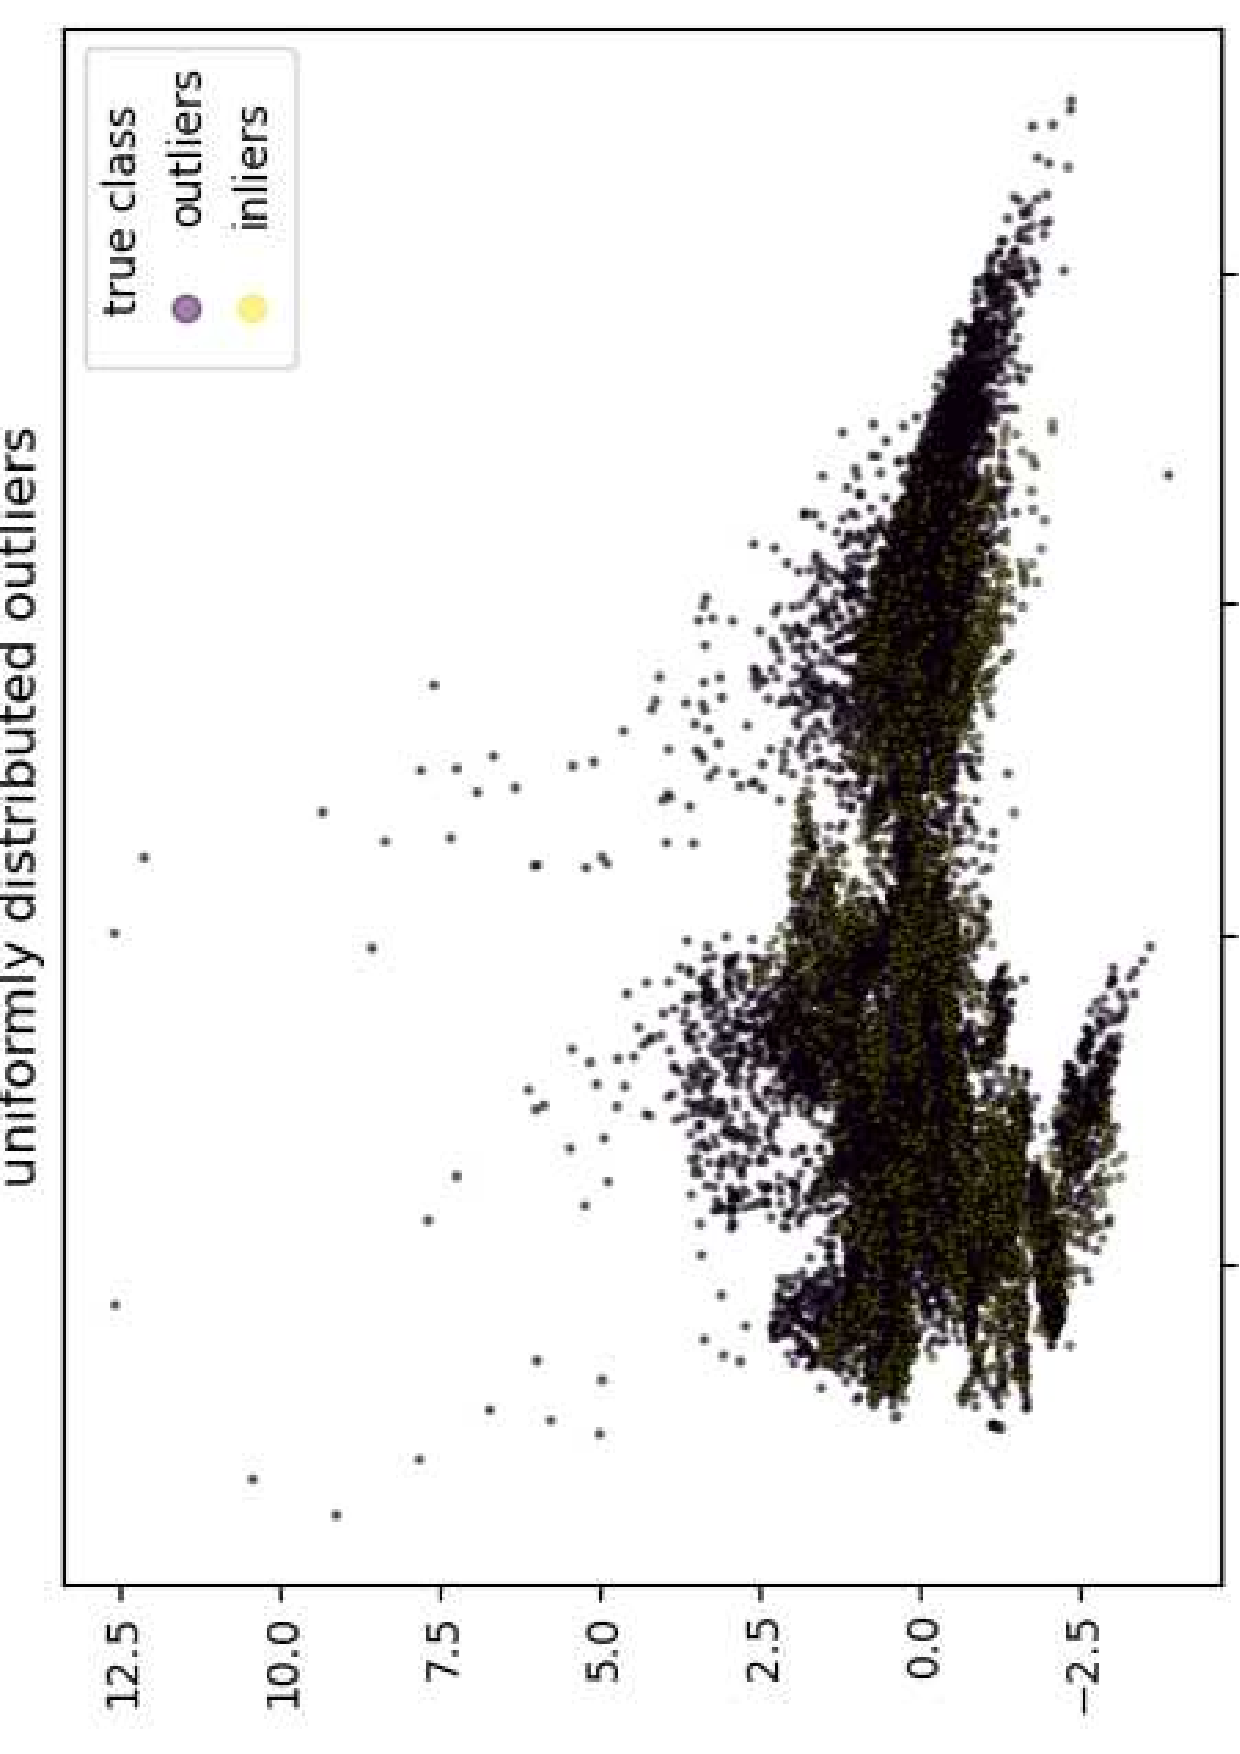
\includegraphics[angle=-90,scale=0.4]
    {manual/images/graph_a.pdf}
  \caption{An example graph in PDF format.}
  \label{fig:SimpleFigure}
\end{figure}

Note that you normally have to give the full path of an image in the \LaTeX{} project tree in order for it to be retrieved and loaded successfully.
We are recommending for each chapter folder create an  \emph{images} or  \emph{figures} folder and upload figures into this folder. Then, in the command \verb|includegraphics{}|, you need to give the full path to that image file. 
More information on creating and formatting figures can be found at \url{https://www.overleaf.com/learn/how-to/Including_images_on_Overleaf}.


%%%%%%%%%%%%%%%%%%%%%%%%%%%%%%%%%%%%%%%%%%%%%%%%%%%%%%%%%%%%%%%%%%%%
\subsection{Raster vs Vector format}
\label{sec:RasterVsVector}

\Cref{fig:RasterVsVector} shows what appears to be twice the same figure. However, the top one is rasterized (i.e., it is a grid of pixels) and is 83Kb in size, while the second is vectorized (i.e., canvas filled with shapes, including text) and is only 32Kb in size. 
The benefit of vectorized is not just the (generally) reduced size but also that it does not pixelate when zooming on it.

\begin{figure}[!ht]
    \centering
    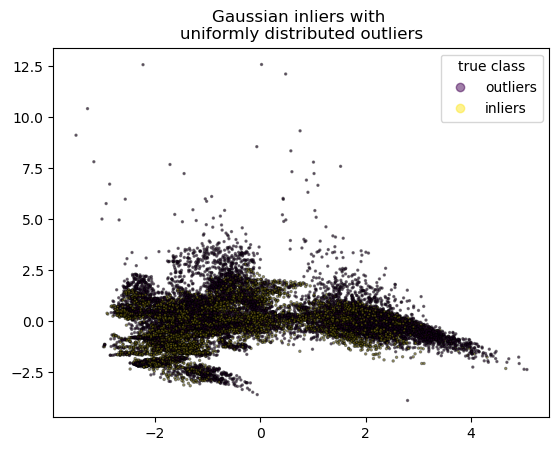
\includegraphics[width=0.8\textwidth]{manual/images/graph_a.png}
    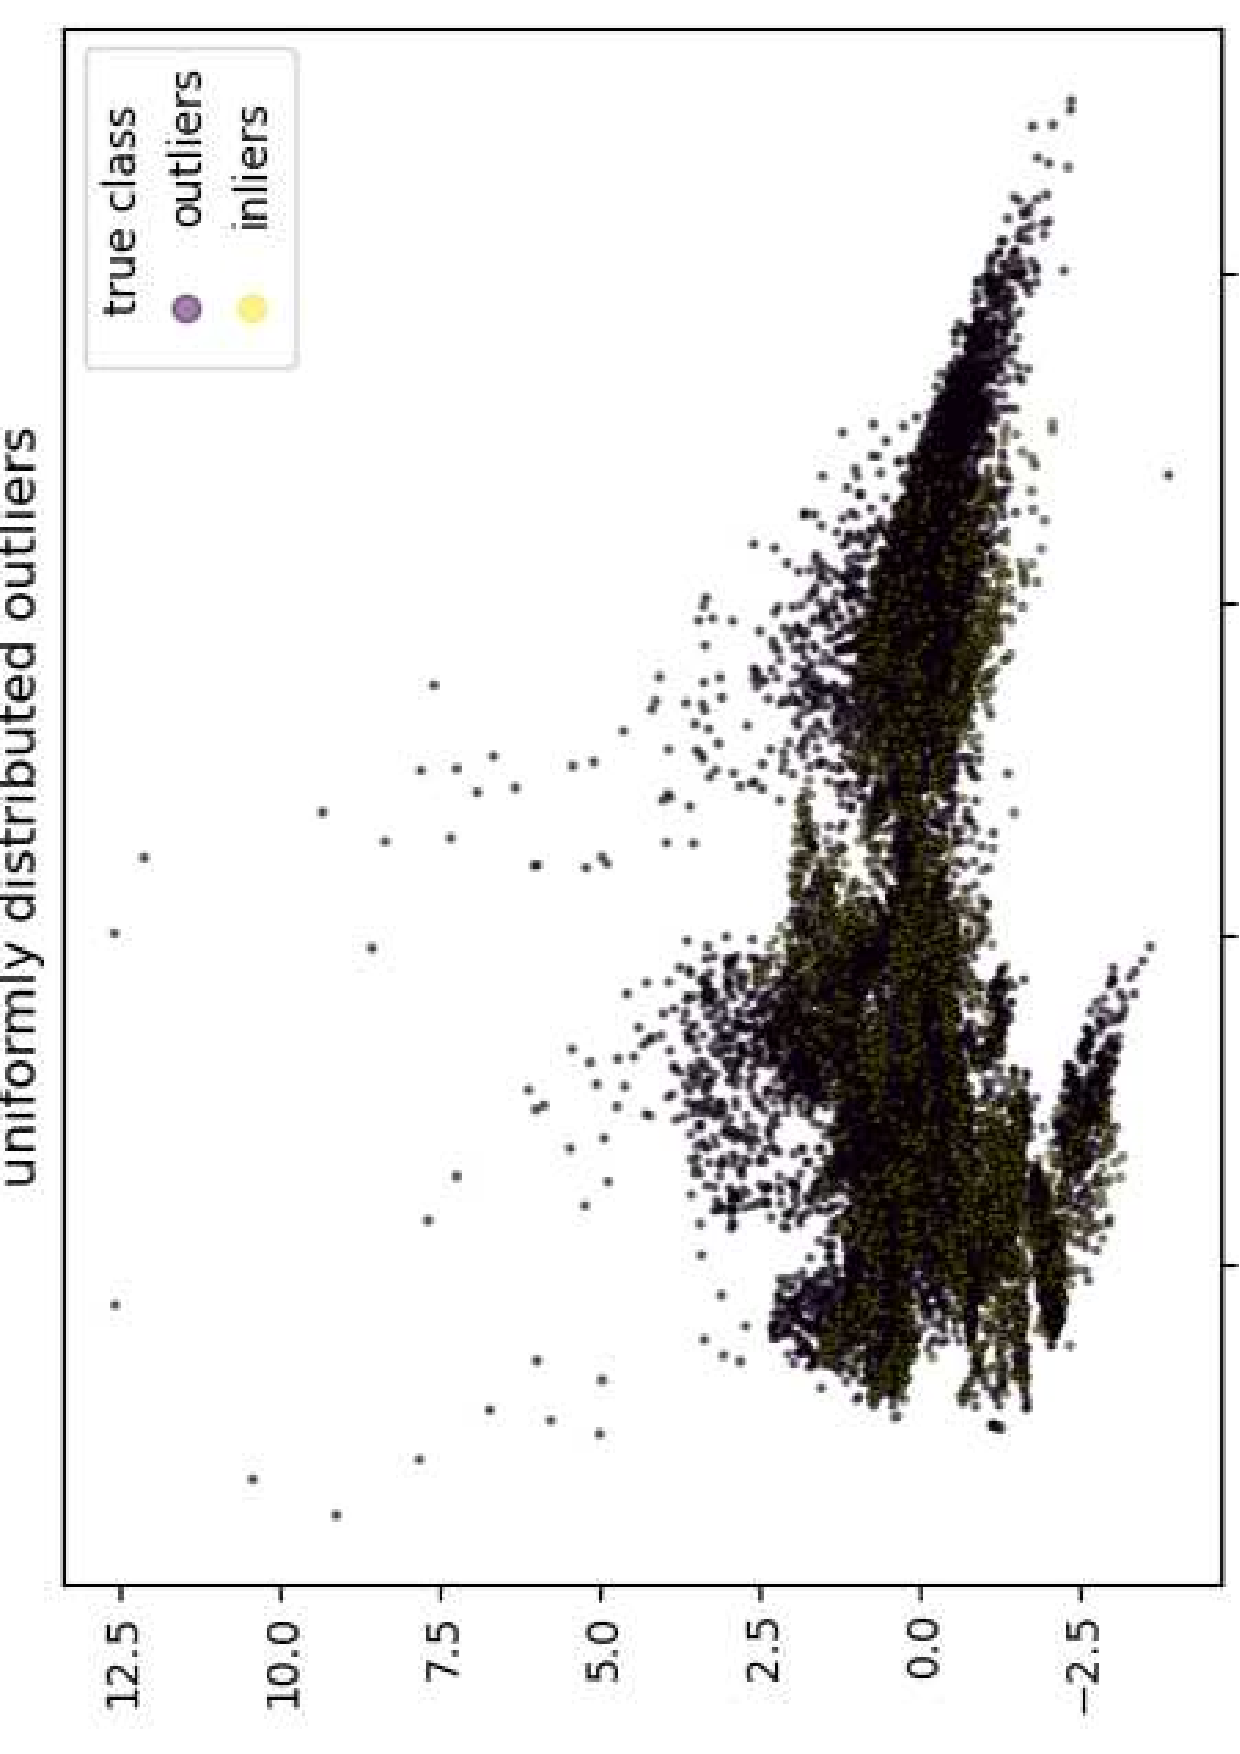
\includegraphics[angle=-90,width=0.8\textwidth]{manual/images/graph_a.pdf}
    \caption{My caption text}
    \label{fig:RasterVsVector}
\end{figure}

WARNING: ".eps" and ".pdf" are common formats used in LaTeX for vectorized images. However, having this file type does \textbf{not} necessarily mean that the content is vectorized.
For example, it is possible to save a ".png" picture of a graph into ".pdf". 
This does not magically transfer the picture into a vectorized image.

Useful software packages to create diagrams and vector images:
\begin{itemize}
    \item Draw.io (opensource): create diagrams (save EPS, or PDF)
    \item MS Powerpoint: create diagrams (save PDF)
    \item Inkscape (opensource): to manipulate vector file (e.g. crop PDF image from MS Powerpoint to fit content).
\end{itemize}


%%%%%%%%%%%%%%%%%%%%%%%%%%%%%%%%%%%%%%%%%%%%%%%%%%%%%%%%%%%%%%%%%%%%
\subsection{LaTeX-generated figure}
\label{sec:LaTeXFigure}

It is also possible to create diagrams in LaTeX using the package \verb|tikz| (which is already loaded for you in this template).
Here, only the data is supplied, and LaTeX code is used to create a diagram/figure layout and present the data content.
The advantage of this approach is that font and font sizing are set in coherence with that of the rest of the document.
However, it is quite tedious to create graphs/diagrams like that.

\Cref{fig:tikz} is an example of figure generated using the drawing package \verb|tikz|.

\begin{figure}
 \centering
 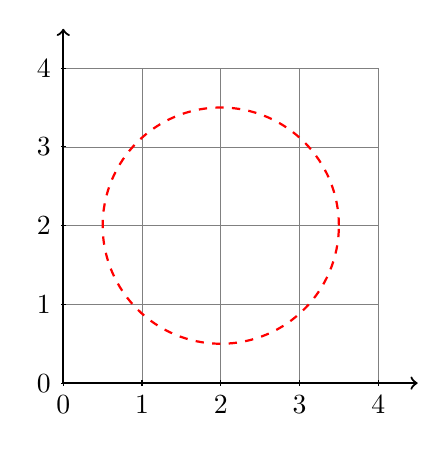
\begin{tikzpicture}
  \draw[step=1cm,gray,very thin] (0,0) grid (4,4);
  \draw[thick,->] (0,0) -- (4.5,0);
  \draw[thick,->] (0,0) -- (0,4.5);
  \foreach \x in {0,1,2,3,4}
   \draw (\x cm,1pt) -- (\x cm,-1pt) node[anchor=north] {$\x$};
  \foreach \y in {0,1,2,3,4}
   \draw (1pt,\y cm) -- (-1pt,\y cm) node[anchor=east] {$\y$};
   \draw[red,thick,dashed] (2,2) circle (1.5cm);
 \end{tikzpicture}
 \caption{A diagram generated using the TikZ package.}
 \label{fig:tikz}
\end{figure}


%%%%%%%%%%%%%%%%%%%%%%%%%%%%%%%%%%%%%%%%%%%%%%%%%%%%%%%%%%%%%%%%%%%%
\subsection{Sub-figures}
\label{sec:SubFigures}

It is possible to create figures with subfigures. 
This requires the use of the packages \verb|caption| and \verb|subcaption| (which are already loaded for you in this template).

Usage is shown in \Cref{fig:Subfigures}. 
You can see both subfigures have labels, which means you can cross-reference them individually in the text as \Cref{fig:Subfigure1} and \Cref{fig:Subfigure2} (see \Cref{sec:crossreferencing} for details on cross-referencing).
More details on how to create a figure with subfigures can be found at \url{https://www.overleaf.com/learn/latex/How_to_Write_a_Thesis_in_LaTeX_(Part_3)\%3A_Figures\%2C_Subfigures_and_Tables}.


\begin{figure}[!ht]
     \centering
     \begin{subfigure}[b]{0.45\textwidth}
         \centering
         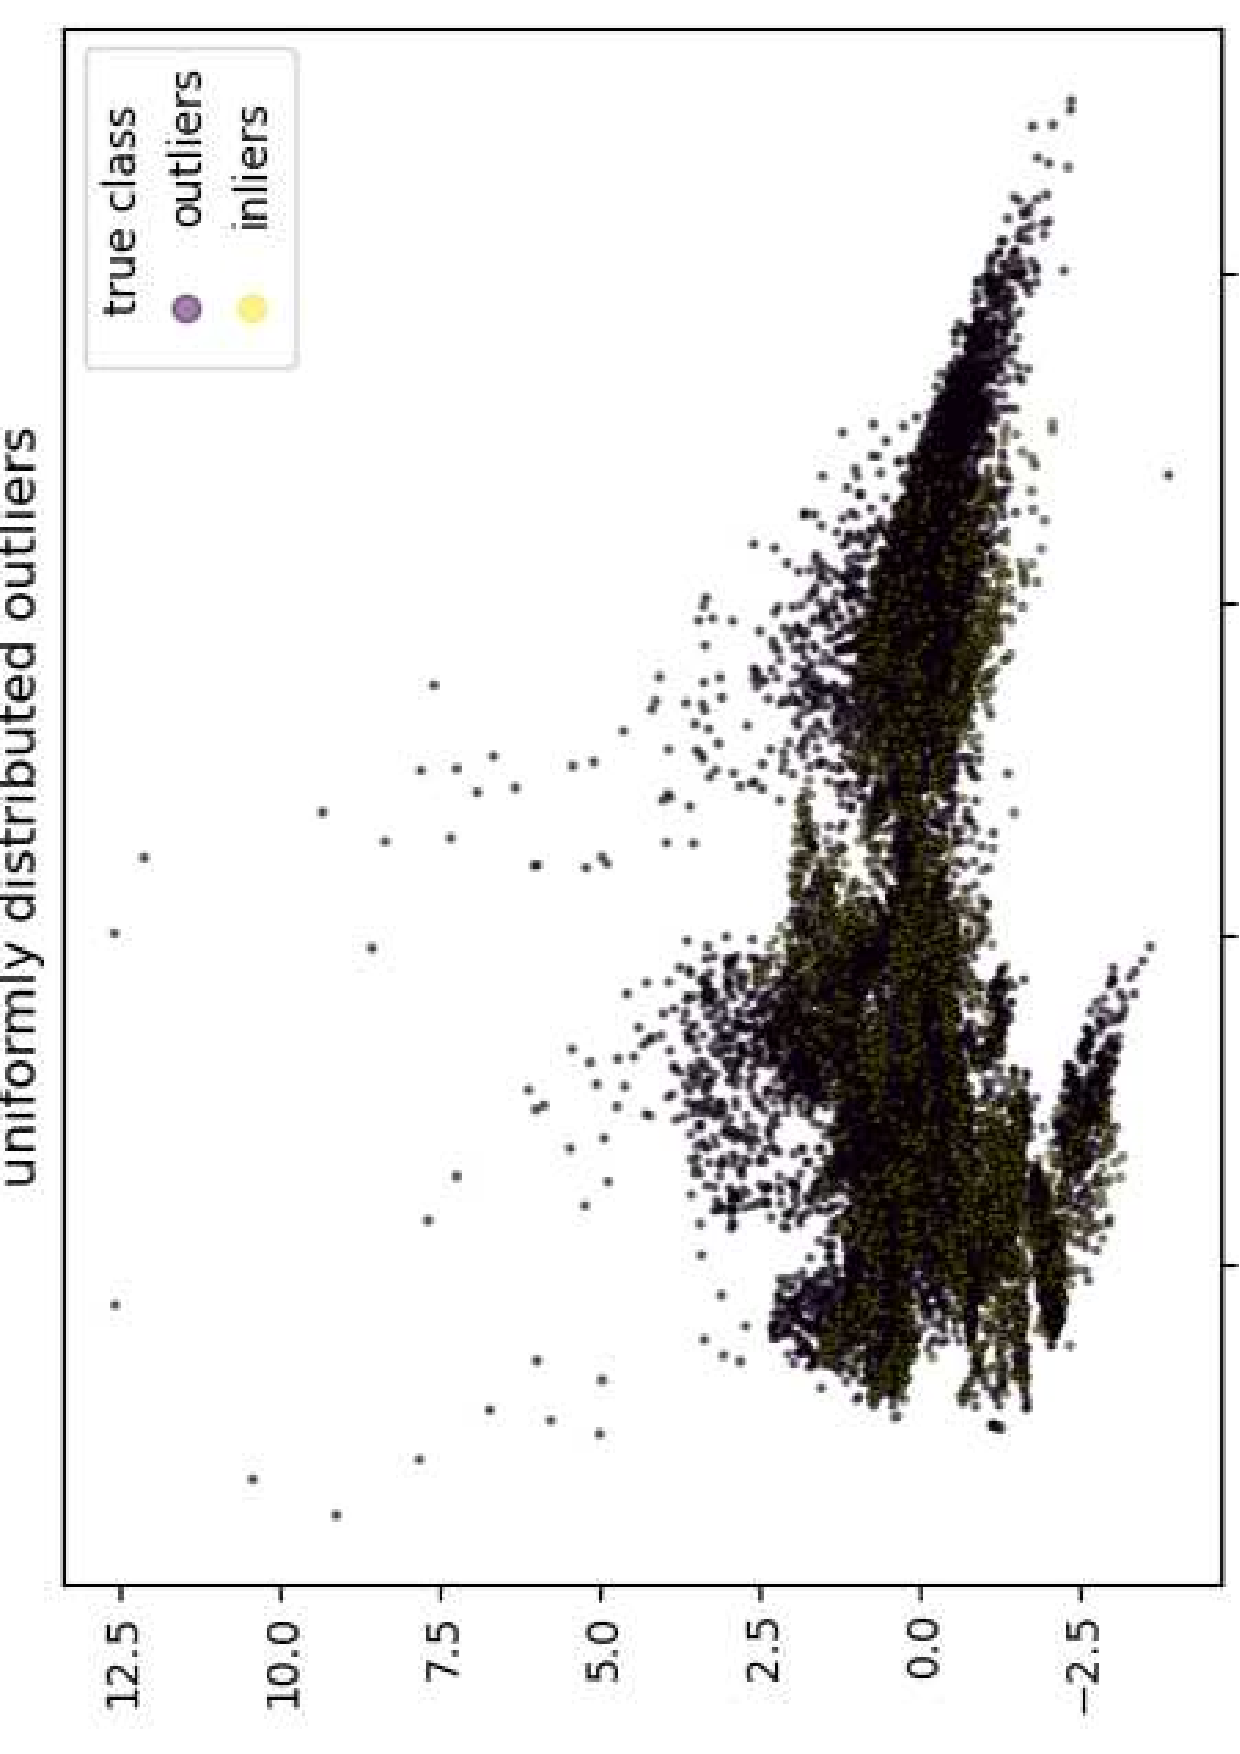
\includegraphics[angle=-90,width=\textwidth]{manual/images/graph_a.pdf}
         \caption{Caption of subfigure 1}
         \label{fig:Subfigure1}
     \end{subfigure}
     \hfill
     \begin{subfigure}[b]{0.45\textwidth}
         \centering
         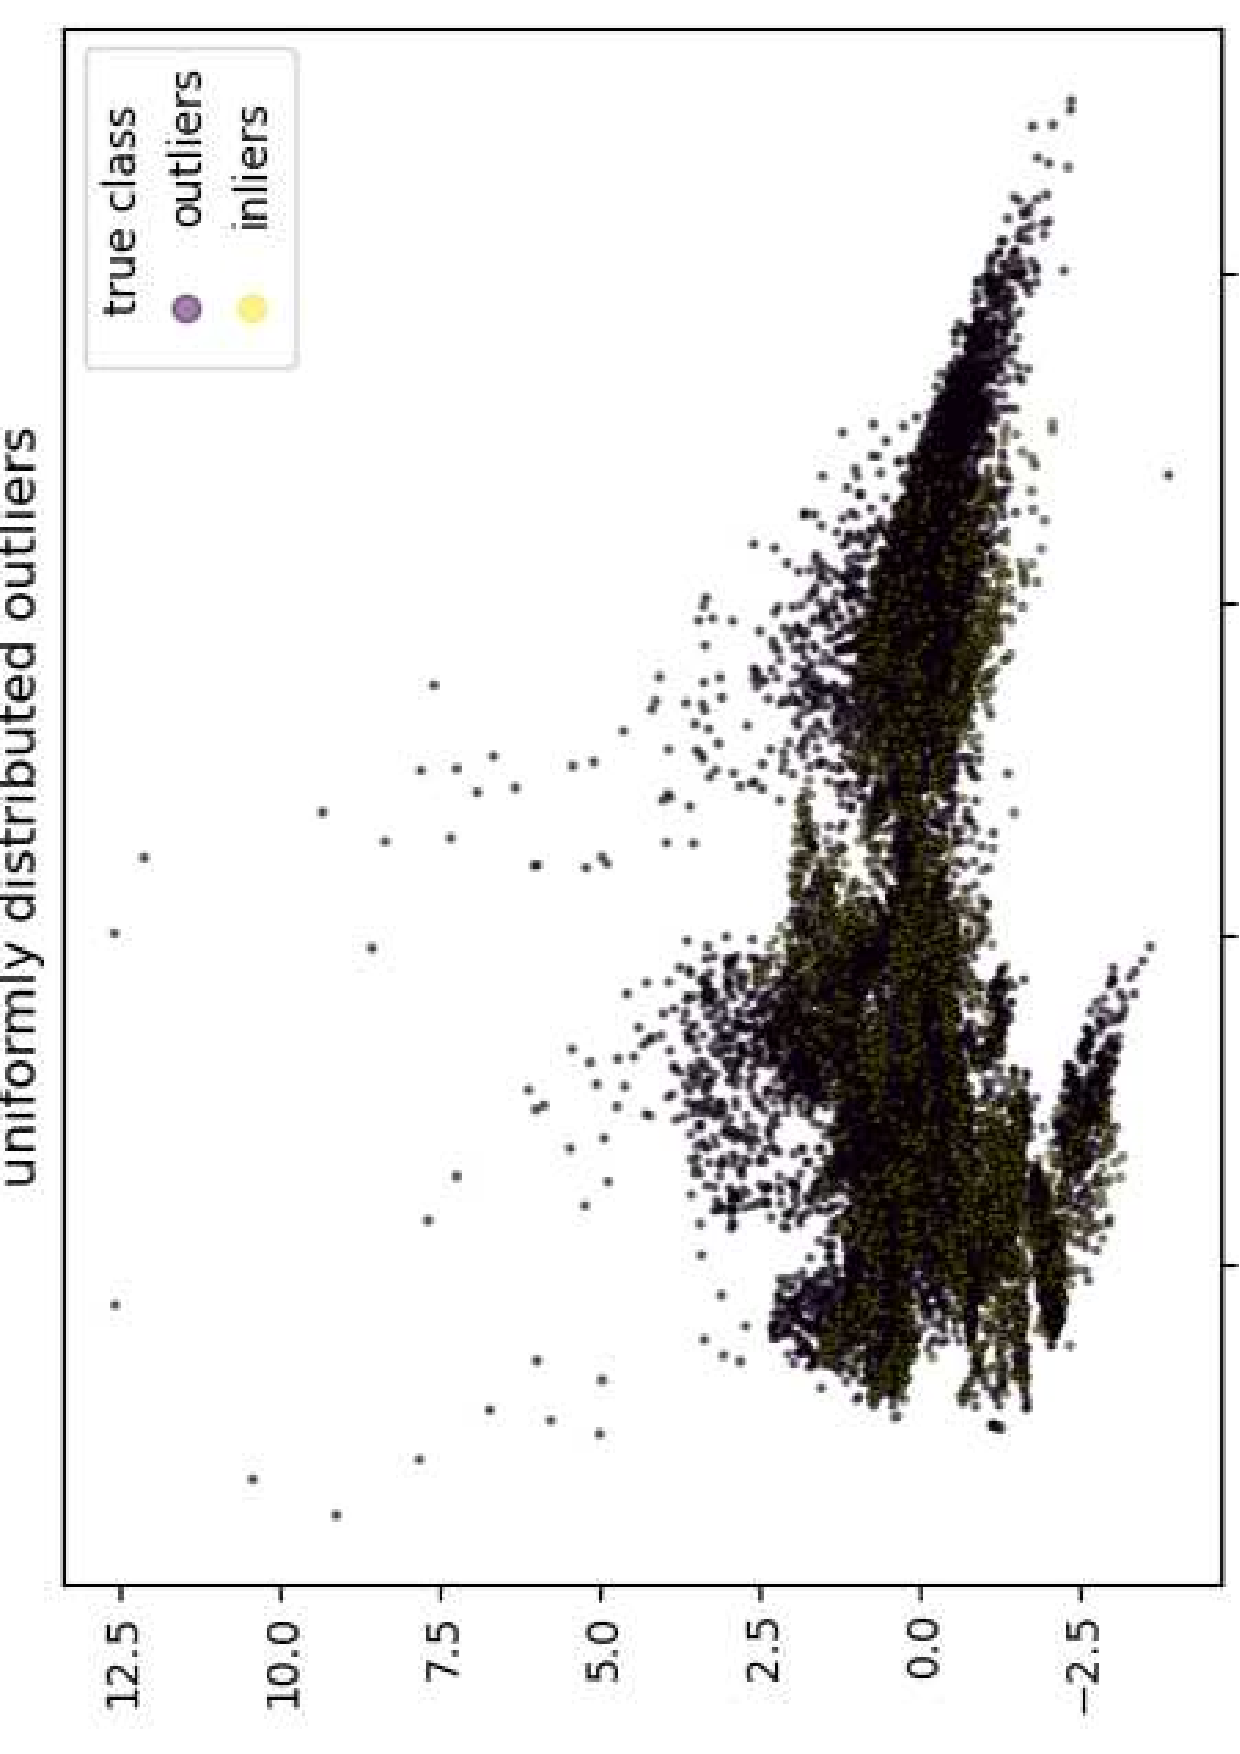
\includegraphics[angle=-90,width=\textwidth]{manual/images/graph_a.pdf}
         \caption{Caption of subfigure 2}
         \label{fig:Subfigure2}
     \end{subfigure}
     \caption{Caption of overall figure}
     \label{fig:Subfigures}
\end{figure}


%%%%%%%%%%%%%%%%%%%%%%
\subsection{And more...}
\label{sec:FiguresMore}

Many other formatting/typesetting options exist. 
For example, you can put a figure in landscape mode using the environment \verb|sidewayfigure| provided by the package \verb|rotating|.

More information on how to create and format figures can be found at \url{https://www.overleaf.com/learn/latex/Inserting_Images}.
But, once again, if you have any specific need, we recommend you search for solutions at the locations suggested in \Cref{sec:Resources} or by using your favorite search engine.



%%%%%%%%%%%%%%%%%%%%%%%%%%%%%%%%%%%%%%%%%%%%%%%%%%%%%%%%%%%%%%%%%%%%%%%%%%%%%%%%%%%%%%%%%%%
\section{Tables}
\label{sec:Tables}

%%%%%%%%%%%%%%%%%%%%%%%%%%%%%%%%%%%%%%%%%%%%%%%%%%%%%%%%%%%%%%%%%%%%
\subsection{Simple Table}
\label{sec:SimpleTable}

The lines below show an example of \LaTeX{} code to create an environment that defines a table \verb|graph_a.pdf|, gives it a caption, and centers everything.
It also gives the table a label so that it can be easily cross-referenced in the text. The table produced by that code is also shown as \Cref{tab:MyFirstTable}.

\begin{verbatim}
\begin{table}[!ht]
    \centering
    \begin{tabular}{|c c c c|} 
    \hline
    Col1 & Col2 & Col2 & Col3 \\
    \hline
    1 & 6 & 87837 & 787 \\ 
    2 & 7 & 78 & 5415 \\
    3 & 545 & 778 & 7507 \\
    4 & 545 & 18744 & 7560 \\
    5 & 88 & 788 & 6344 \\
    \hline
    \end{tabular}
    \caption{Table to test captions and labels.}
    \label{tab:MyFirstTable}
\end{table}
\end{verbatim}

\begin{table}[!ht]
    \centering
    \begin{tabular}{|c c c c|} 
    \hline
    Col1 & Col2 & Col2 & Col3 \\
    \hline
    1 & 6 & 87837 & 787 \\ 
    2 & 7 & 78 & 5415 \\
    3 & 545 & 778 & 7507 \\
    4 & 545 & 18744 & 7560 \\
    5 & 88 & 788 & 6344 \\
    \hline
    \end{tabular}
    \caption{Table to test captions and labels.}
    \label{tab:MyFirstTable}
\end{table}

In this code, the \emph{table} environment (i.e. \verb|\begin{table}...\end{table}|) creates a floating environment of the type 'table' that can be given a caption and a label. 
\verb|\centering| centers the table inside that table floating environment. 
Then, the \emph{tabular} environment is the environment that contains the description of the table. 
The tabular environment argument tells \LaTeX{} the alignment to be used in each column and the vertical lines to insert. 
In the table above, \verb!|c c c c|! defines a table with four columns in all of which the text is centered. 
Inside the \emph{tabular} environment, \verb|\hline| creates a horizontal line through the table (you can use the command \verb|\cline{...}| to make a horizontal line that only spans a subset of the columns). Finally, each row of data is entered with the cell content delimited with the character \verb|&| and the end of the row marked with the characters \verb|\\|.


%%%%%%%%%%%%%%%%%%%%%%%%%%%%%%%%%%%%%%%%%%%%%%%%%%%%%%%%%%%%%%%%%%%%
\subsection{Merging Rows and Columns}
\label{sec:TableRowMerging}

If you wish to merge some cells together horizontally or vertically, use the \verb|\multicolumn{...}|) or \verb|\multirow{...}| commands, the latter requiring the \verb|multirow| package (which already loaded for you in this template).
\Cref{tab:MySecondTable} shows an example of table containing both merges columns and merged cells.

\begin{table}[!ht]
    \centering
    \caption{Table with merged cells.}
    \label{tab:MySecondTable}
    \begin{tabular}{|cccc|} 
    \hline
    Col1 & Col2 & Col2 & Col3 \\
    \hline
    \multicolumn{2}{|c}{7} & 87837 & 787 \\  
    \multirow{2}{*}{5} & 7 & 78 & 5415 \\ 
    & 545 & 778 & 7507 \\
    4 & 545 & 18744 & 7560 \\
    5 & 88 & 788 & 6344 \\
 \hline
 \end{tabular}
\end{table}

If you have to insert a very long table, which takes up two or more pages in your document, use the \emph{longtable} package (already loaded for you in this template). If you wish to have your table in landscape mode, consider using the \emph{sidewaystable} or \emph{landscape} packages.  

More information on how to create and format tables (including how to color rows/cells) can be found at \url{https://www.overleaf.com/learn/latex/Tables} and many other places at the resources listed in \Cref{sec:Resources} and elsewhere on the web.




%%%%%%%%%%%%%%%%%%%%%%%%%%%%%%%%%%%%%%%%%%%%%%%%%%%%%%%%%%%%%%%%%%%%
\subsection{Column Widths}
\label{sec:TableColumnWidths}

As mentioned, in the tables above, \verb!|c c c c|! defines a table with four columns in all of which the text is centered (it also instructs that double vertical lines should bind the table on the left and right).
However, as illustrated in \Cref{tab:MyThirdTable1}, the width of each column expands in order to accommodate the largest width of the content of any of its cells; there is no text wrapping.

To address this, you can replace the first \verb|c| with \verb|p{0.2\textwidth}| which forces the first column to have a width of no more than $20\%$ of the text width, which triggers some text wrapping in this case.
This approach is illustrated with the first column of \Cref{tab:MyThirdTable}.
However, note that the content of the cells in that column is not centred anymore. 
To retain text centering, \verb|p{0.2\textwidth}| needs to be prepended by \verb|>{\centering}|, which is illustrated for the second column of \Cref{tab:MyThirdTable}.

\begin{table}[!ht]
    \centering
    \caption{Table with fixed column widths.}
    \label{tab:MyThirdTable1}
    \begin{tabular}{|c c c c|} 
    \hline
    Col1 & Col2 & Col2 & Col3 \\
    \hline
    1 & 6 & 87837 & 787 \\  
    Best table in the world & 7 & 78 & 5415 \\ 
    3 & 545 & 778 & 7507 \\
    4 & 545 & 18744 & 7560 \\
    5 & 88 & 788 & 6344 \\
    \hline
    \end{tabular}
\end{table}

\begin{table}[!ht]
    \centering
    \caption{Table with fixed column widths.}
    \label{tab:MyThirdTable}
    \begin{tabular}{|p{0.2\textwidth}>{\centering}p{0.2\textwidth}cc|} 
    \hline
    Col1 & Col2 & Col2 & Col3 \\
    \hline
    1 & 6 & 87837 & 787 \\  
    Best table in the world & 7 & 78 & 5415 \\ 
    3 & 545 & 778 & 7507 \\
    4 & 545 & 18744 & 7560 \\
    5 & 88 & 788 & 6344 \\
    \hline
    \end{tabular}
\end{table}





%%%%%%%%%%%%%%%%%%%%%%%%%%%%%%%%%%%%%%%%%%%%%%%%%%%%%%%%%%%%%%%%%%%%
\subsection{Colouring Cells}
\label{sec:TableColouring}

You may wish to color cells in a table you created.
This can be done by loading the package \verb|xcolor| (already loaded for you in this template), and using the \verb|cellcolor{...}| command in the cell to be coloured.
This is illustrated in \Cref{tab:MyFourthTable}.

It is also possible to color an entire column at once.
This requires defining a new column type.
\Cref{tab:MyFifthTable} illustrates this with the new column type \verb|G| define in the preamble of this \LaTeX{} document as:

\begin{verbatim}
\newcolumntype{G}{>{\centering\columncolor{blue!20!white}}p{0.2\textwidth}}
\end{verbatim}


\begin{table}[!ht]
    \centering
    \caption{Table with coloured cell.}
    \label{tab:MyFourthTable}
    \begin{tabular}{|cccc|} 
    \hline
    Col1 & Col2 & Col2 & Col3 \\
    \hline
    1 & 6 & 87837 & 787 \\  
    2 & \cellcolor{blue} 7 & 78 & 5415 \\ 
    3 & 545 & 778 & 7507 \\
    4 & 545 & 18744 & 7560 \\
    5 & 88 & 788 & 6344 \\
    \hline
    \end{tabular}
\end{table}

%Define this command in preamble to use it in whole document
\newcolumntype{G}{>{\centering\columncolor{blue!20!white}}p{0.2\textwidth}}
\begin{table}[!ht]
    \centering
    \caption{Table with coloured column.}
    \label{tab:MyFifthTable}
    \begin{tabular}{||cGcc||} 
    \hline
    Col1 & Col2 & Col2 & Col3 \\
    \hline\hline
    1 & 6 & 87837 & 787 \\  
    2 & 7 & 78 & 5415 \\ 
    3 & 545 & 778 & 7507 \\
    4 & 545 & 18744 & 7560 \\
    5 & 88 & 788 & 6344 \\
 \hline
 \end{tabular}
\end{table}



%%%%%%%%%%%%%%%%%%%%%%%%%%%%%%%%%%%%%%%%%%%%%%%%%%%%%%%%%%%%%%%%%%%%
\subsection{Multipage Table}
\label{sec:TableMultipage}

When typesetting a table, you may come across a table whose content makes it span more than a page. 
\LaTeX{} does not handle these situations, by splitting the table automatically across two (or more) pages.
Instead, you have to change your table environment to a \verb|longtable| environment and provide the necessary information whether and how to repeat the table caption on each page, repeat the column headers, etc. 
How this is achieved is illustrated with \Cref{tab:TableLong}.


\begin{longtable}{|l|l|l|}
    \caption{A sample long table.} 
    \label{tab:TableLong} \\
    
    \hline 
    \textbf{First column} & \textbf{Second column} & \textbf{Third column} \\ 
    \hline 
    \endfirsthead
    
    \multicolumn{3}{c}{{\tablename\ \thetable{} -- continued from previous page}} \\
    \hline 
    \textbf{First column} & \textbf{Second column} & \textbf{Third column} \\ 
    \hline 
    \endhead
    
    
    \hline \multicolumn{3}{|r|}{{Continued on next page}} \\ \hline
    \endfoot
    
    \hline \hline
    \endlastfoot

One & abcdef ghjijklmn & 123.456778 \\
One & abcdef ghjijklmn & 123.456778 \\
One & abcdef ghjijklmn & 123.456778 \\
One & abcdef ghjijklmn & 123.456778 \\
One & abcdef ghjijklmn & 123.456778 \\
One & abcdef ghjijklmn & 123.456778 \\
One & abcdef ghjijklmn & 123.456778 \\
One & abcdef ghjijklmn & 123.456778 \\
One & abcdef ghjijklmn & 123.456778 \\
One & abcdef ghjijklmn & 123.456778 \\
One & abcdef ghjijklmn & 123.456778 \\
One & abcdef ghjijklmn & 123.456778 \\
One & abcdef ghjijklmn & 123.456778 \\
One & abcdef ghjijklmn & 123.456778 \\
One & abcdef ghjijklmn & 123.456778 \\
One & abcdef ghjijklmn & 123.456778 \\
One & abcdef ghjijklmn & 123.456778 \\
One & abcdef ghjijklmn & 123.456778 \\
One & abcdef ghjijklmn & 123.456778 \\
One & abcdef ghjijklmn & 123.456778 \\
One & abcdef ghjijklmn & 123.456778 \\
One & abcdef ghjijklmn & 123.456778 \\
One & abcdef ghjijklmn & 123.456778 \\
One & abcdef ghjijklmn & 123.456778 \\
One & abcdef ghjijklmn & 123.456778 \\
One & abcdef ghjijklmn & 123.456778 \\
One & abcdef ghjijklmn & 123.456778 \\
One & abcdef ghjijklmn & 123.456778 \\
\end{longtable}





%%%%%%%%%%%%%%%%%%%%%%%%%%%%%%%%%%%%%%%%%%%%%%%%%%%%%%%%%%%%%%%%%%%%%%%%%%%%%%%%%%%%%%%%%%%
\section{Mathematical Expressions}
\label{sec:Math}

%%%%%%%%%%%%%%%%%%%%%%%%%%%%%%%%%%%%%%%%%%%%%%%%%%%%%%%%%%%%%%%%%%%%%%%%%%%%%%%
\subsection{Inline vs Display Mode}
\label{sec:MathModes}

Mathematical expressions, including formulas, can be entered in two different ways: \emph{inline} mode or \emph{display} mode. 
Inline mode means that the mathematical expression will appear within the text; display mode means that it will appear in a separate line (or set of lines).

You can use two types of delimiters to typeset mathematical expressions in inline mode, \verb|\(...\)| or \verb|$...$|, or the \emph{math} environment \verb|\begin{math}...\end{math}|. 
Two examples of inline mathematical expressions are \(d=\sqrt{x^2+y^2}\) and $M = A + B$.

You can use the delimiters \verb|\[...\]| or the \emph{displaymath} \emph{equation} or \emph{align} environments \verb|\begin{equation}| \verb|...\end{equation}| to typeset mathematical expressions in display mode.

An example of mathematical expression in display mode is: \[d=\sqrt{x^2+y^2}\]

An example of mathematical expression in display mode is: \begin{displaymath}d=\sqrt{x^2+y^2}\end{displaymath}

An example of mathematical expression in display mode is: \begin{equation}d=\sqrt{x^2+y^2}\end{equation}



%%%%%%%%%%%%%%%%%%%%%%%%%%%%%%%%%%%%%%%%%%%%%%%%%%%%%%%%%%%%%%%%%%%%
\subsection{Mathematical Symbols and Greek letters}
\label{sec:MathSymbols}

You can use an extremely broad range of Greek letters and mathematical symbols, such as:
\begin{itemize}[nosep]
  \item Binary operators: $\times \otimes \oplus \cup \cap$ 
  \item Relation operators: $< > \subset \supset \subseteq \supseteq$
  \item Greek letters: $\alpha \beta \gamma \rho \sigma \delta \epsilon$, and $A B \Gamma \Sigma \Delta E$
  \item Other: $\int \oint \sum \prod$
\end{itemize}
%
A first list of mathematical symbols can be found at \url{https://www.overleaf.com/learn/latex/List_of_Greek_letters_and_math_symbols} with an even more detailed list of symbols available at \url{https://oeis.org/wiki/List_of_LaTeX_mathematical_symbols}.


%%%%%%%%%%%%%%%%%%%%%%%%%%%%%%%%%%%%%%%%%%%%%%%%%%%%%%%%%%%%%%%%%%%%
\subsection{Equation}
\label{sec:MathEquations}

\LaTeX{} is extremely powerful in general, but in particular when it comes to typesetting mathematical expressions, such as equations. 
The equation below is just one example. 
As you can see, 

\begin{align}\label{eq:MyEquation}
\begin{split}
S(\omega) 
&= \frac{\alpha g^2}{\omega^5} e^{[ -0.74\bigl\{\frac{\omega U_\omega 19.5}{g}\bigr\}^{\!-4}\,]} \\
&= \frac{\alpha g^2}{\omega^5} \exp\Bigl[ -0.74\Bigl\{\frac{\omega U_\omega 19.5}{g}\Bigr\}^{\!-4}\,\Bigr] 
\end{split}
\end{align}


%%%%%%%%%%%%%%%%%%%%%%
\subsection{And more...}
\label{sec:MathMore}

Further details about typesetting mathematical expressions can be found at \url{https://www.overleaf.com/learn/latex/Mathematical_expressions}.




%%%%%%%%%%%%%%%%%%%%%%%%%%%%%%%%%%%%%%%%%%%%%%%%%%%%%%%%%%%%%%%%%%%%%%%%%%%%%%%%%%%%%%%%%%%
\section{Properly Typesetting Units}

In any scientific and engineering piece of work units play a major part. Without them our numerical information is practically useless. We need to be able to properly typeset them as in publishing, they often do follow specific rules that, sadly, most of the time, simple word processing packages ignore. Units, for example, are not set in italics or in random fonts that we seem to be using.

There are many \LaTeX{} packages you can use and explore to help you typeset units properly, but in this template, we use the \verb|siunitx| package. 

For example, \verb|\unit{kg.m.s^{-1}}| produces \unit{kg.m.s^{-1}}. \\
\verb|\unit{\kilogram\metre\per\second}| produces the same output \unit{\kilogram\metre\per\second}.

If you want to nicely refer to an angle you can just type \verb|\ang{10}| to get \ang{10} or \verb|\ang{3;23;5}| for \ang{3;23;5} or type \verb|\qty{3}{mm}| for \qty{3}{mm} or more explicitly \verb|\qty{3}{\milli\metre}| for the same effect as \qty{3}{\milli\metre}. 
\verb|\qtylist{5;10;15}{\metre}| will produce nicely \qtylist{5;10;15}{\metre}. 
\verb|\qtyproduct{5 x 10 x 15}{\metre}| produces \qtyproduct{5 x 10 x 15}{\metre}.


The options are very comprehensive, and no matter how complex or simple your units are they will be typeset properly and beautifully.
Detailed instructions on how to use the various commands that the \verb|siunitx| package makes available for typesetting units properly are given in \url{https://mirror-hk.koddos.net/CTAN/macros/latex/contrib/siunitx/siunitx.pdf}



%%%%%%%%%%%%%%%%%%%%%%%%%%%%%%%%%%%%%%%%%%%%%%%%%%%%%%%%%%%%%%%%%%%%%%%%%%%%%%%%%%%%%%%%%%%
\section{Cross-referencing}
\label{sec:crossreferencing}

Your work will have internal references to various objects like equations, figures, chapters, sections, etc. Let's have a look at some examples.

Using the readily available command \verb|\ref{}|, you can automatically reference such objects. For example:
\begin{itemize}
    \item \verb|Section~\ref{sec:Figures}| typesets `Section~\ref{sec:Figures}'
    \item \verb|Figure~\ref{fig:SimpleFigure}| typesets `Figure~\ref{fig:SimpleFigure}'
    \item \verb|Table~\ref{tab:MyFirstTable}| typesets `Table~\ref{tab:MyFirstTable}'
    \item \verb|Equation \ref{eq:sedov}| typesets `Equation \ref{eq:MyEquation}'
\end{itemize}

However, \verb|\ref{}| requires you to actually type the type of object referenced, i.e.,  \verb|Section| in \verb|Section~\ref{sec:Figures}| in order to obtain `Section~\ref{sec:Figures}'. 
A smart and easier way to cross-reference is to use the \verb|cleveref| package (already loaded for you in this template).
The \verb|cleveref| package provides the commands \verb|\cref{}|, \verb|\Cref{}|, \verb|\crefrange{}|, and many more. For example:
\begin{itemize}
    \item \verb|\cref{sec:Figures}| typesets `\cref{sec:Figures}' and \verb|\cref{tab:MyFirstTable}| typesets `\cref{tab:MyFirstTable}'
    \item \verb|\Cref{sec:Figures}| typesets `\Cref{sec:Figures}'
    \item \verb|\cref{sec:Figures,sec:Math}| typesets `\cref{sec:Figures,sec:Math}'
    \item \verb|\crefrange{sec:Figures}{sec:Math}| typesets `\crefrange{sec:Figures}{sec:Math}'
\end{itemize}
%
These commands automatically identify the type of each referenced object and ensure that those types are typeset consistently throughout the document.

Although \LaTeX{} does not require it, it is good practice to try and name labels by giving an indication of what they represent, such as \verb|\label{sec:...}| for labels of sections and sub-sections.
This way, they can be retrieved easily and not be confused.




%%%%%%%%%%%%%%%%%%%%%%%%%%%%%%%%%%%%%%%%%%%%%%%%%%%%%%%%%%%%%%%%%%%%%%%%%%%%%%%%%%%%%%%%%%%
\section{Bibliography and Citations}
\label{sec:Bibligraphy}

Citations of works that support your arguments and are used to reference and acknowledge the original sources of information that you use, discuss, or develop are very easy. 

\LaTeX{} uses a specific methodology to describe and process lists of references: Bibtex (\url{http://www.bibtex.org}).
Bibtex manifest itself in your \LaTeX{} project in the form of a file with extension \verb|.bib| and requires loading the package \verb|natbib| to be able to process \verb|.bib| files and typeset the information they contain.
In the current project, the file is called \verb|thesis_bibliography.bib|.
The file has a simple text format and essentially contains a database of entries.
The most common entry is for an \verb|@article|, but there are many more, as can be seen in the example file \verb|thesis_bibliography.bib|. 
What is important is that every entry you create has its own unique label that is then used to \emph{cite} the entry appropriately in your \LaTeX{} text and create the list of references that is created automatically and included at the end of our thesis.

Citations in the text are made using the commands \verb|\citet| and \verb|\citep| and possibly \verb|\citeauthor| or other forms of citation commands useful for more specific cases.
For example, "\citet{demoArticle} provided a comprehensive survey in their review paper" is obtained using the command \verb|\citet{demoArticle}|.
This command creates an entry that has the authors names as part of the sentence (here used as subjects). 
In contrast, "a comprehensive survey is provided in \citep{demoArticle}" is obtained using the command \verb|\citep{demoArticle}|. 
This commands just creates an entry that is just citation to the reference.
Also note that an entry in the list of references, located at the end of the thesis.

You must let \LaTeX{} know where the bib file is that contains the details of the references that you cite in you \verb|tex| file.
This is done by adding the command \verb|\bibliography{file.bib}| in your main \verb|.tex| file.
In this thesis template, \verb|\bibliography{thesis_bibliography.bib}| is added at the end of the \verb|bibiography/bibliography.tex| file.

\LaTeX{}, in combination with its bibliography packages, can create any style of referencing that you might need and more information can be found at  \url{https://www.overleaf.com/learn/latex/Bibliography_management_with_natbib} or using different packages \url{https://www.overleaf.com/learn/latex/Bibliography_management_with_bibtex} or alternatively \url{https://www.overleaf.com/learn/latex/Bibliography_management_with_biblatex}.
% However, for this thesis template, we have already selected the AGSM style (and suggest you keep it) that is defined in the \verb|thesis.tex| file with the command \verb|\bibliographystyle{agsm}|.
However, for this thesis template, we have already selected the abbrvnat style (and suggest you keep it) that is defined in the \verb|/bibiography/bibliography.tex| file with the command \verb|\bibliographystyle{abbrvnat}|.

\textbf{Note:} An emerging alternative to the use of \emph{Bibtex} (used with the \verb|natbib| package) is emerging.
It is called \emph{Biber} (used with the \verb|biblatex| package).
We do not explain here how to work with Biber, but it is, in fact, very similar to working with Bibtex. 
For now, we, however, recommend sticking to Bibtex.

%%%%%%%%%%%%%%%%%%%%%%%%%%%%%%%%%%%%%%%%%%%%%%%%%%%%%%%%%%%%%%%%%%%%%%%%%%%%%%%%%%%%%%%%%%%
\section{Acronyms}
\label{sec:Acronyms}

There are several ways of introducing acronyms. 
In general it is good practice to introduce them in full on first use. 
For example, \verb|\gls{CVRMSE}| produces \gls{CVRMSE}, and it shows in full because 
it is the first time it is being used.
Next usage should not expand as it has already been introduced, as shown next: \gls{CVRMSE}.

Acronyms that are very familiar in the field or self explanatory may not be expanded on any use.
For example, \verb|\acrshort{CO2e}| produces \acrshort{CO2e}.
Some other times, the usage is so sporadic 
(e.g., used in the first chapter and used again 50 pages later)
that you might want to force showing it in full regardless of previous use: 
\verb|\acrfull{CIBSE}| displays \acrfull{CIBSE}
(this comes in handy sometimes for captions of figures and tables to help the reader).
You can even show the definition without using the acronym at all: 
\verb|\acrlong{CIBSE}| produces \acrlong{CIBSE}.